\documentclass[xetex]{beamer}
%\documentclass[draft, xetex]{beamer}

		% Iclude packages and commands used text-wide.	
%%%%%%%%%%%%%%%%%%%%%%%%%%%%%%%%%%%%%%%%%%%%%%%%%%%%%%%%%%%%%%%%%%%%%%%%%%%%%%%%%%%%%%%%%%%%%%%%%%%%%%%%%%%

\usepackage{mystyle}
\usepackage{my_commands}

		% Presentation settings.
%%%%%%%%%%%%%%%%%%%%%%%%%%%%%%%%%%%%%%%%%%%%%%%%%%%%%%%%%%%%%%%%%%%%%%%%%%%%%%%%%%%%%%%%%%%%%%%%%%%%%%%%%%%

	\mode<presentation>{
		%\usetheme{Berlin}
		\usetheme{CambridgeUS}
		\setbeamercovered{transparent}
	}

		% Title
	\title[Parrellel Tempering]{Parrellel Tempering }
	\subtitle{theory and applications}

	%\beamerdefaultoverlayspecification{<+->}
	\date{24 April 2013}
	\author[Łącki]{Mateusz Łącki}
	\institute[UW]{Uniwersytet Warszawski}
	\titlegraphic{\includegraphics[scale=.4, keepaspectratio]{./picts/eagle.jpg}}

	\usefonttheme[onlylarge]{structuresmallcapsserif}
	%\usefonttheme[onlysmall]{structurebold}

		% The document
%%%%%%%%%%%%%%%%%%%%%%%%%%%%%%%%%%%%%%%%%%%%%%%%%%%%%%%%%%%%%%%%%%%%%%%%%%%%%%%%%%%%%%%%%%%%%%%%%%%%%%%%%%%	

\begin{document}
	\fontspec[Numbers={OldStyle}]{Linux Libertine O}

	%%%%%%%%%%%%%%%%%%%%%%%%%%%%%%%%%%%%%%%%%%%%%%%%%%%%%%%%%%%%%%

	\begin{frame}
		\titlepage
	\end{frame}

	\begin{frame}
		\frametitle{Today's Agenda}
		%\tableofcontents[pausesections]
		\tableofcontents
	\end{frame}
	
	%%%%%%%%%%%%%%%%%%%%%%%%%%%%%%%%%%%%%%%%%%%%%%%%%%%%%%%%%%%%%%


	%\section[Why bother?]{Why use parallel tempering?}
	\section[Motivation]{What? Why? Who?}		
			\begin{frame}
		\frametitle{What is Parallel Tempering? Nutshell view.}
	
	\begin{itemize}
		\item Stochastic simulation algorithm
		\item a.k.a. replica exchange Monte Carlo 
		\begin{itemize}	
			\item sampling method  
		\end{itemize}
		\item Extension to Metropolis-Hastings algorithm \dots
		\item \dots or rather Metropolis-Hastings-Green algorithm 
		\begin{itemize}
			\item more abstract version: general kernels
			\item more freedom: discrete kernels, continous kernels, different dimensions  
		\end{itemize} 

	\end{itemize}	

	\begin{center}
		\begin{figure}\includegraphics[scale=.3, keepaspectratio]{./picts/nutshell1.jpg}\end{figure}	
	\end{center}

\end{frame}


\begin{frame}
		\frametitle{Why Parallel Tempering? }
	
	\begin{itemize}
		\item Tool to fight \emph{ multimodality }
		\begin{itemize}
			\item "allows good mixing with multimodial target distributions"
			\item response to Metropolis-Hastings localness    
			\item better estimation of integrals $ \int_{\mathbb{R}^d} f(x) \pi(x) \mathrm{d} x $
		\end{itemize}
		\item[] 

		\item In certain physical models: thermodynamic interpretation
		\begin{itemize}
			\item Gibbs random-field model
		\end{itemize}
	\end{itemize}	

\end{frame}

\begin{frame}
		\frametitle{Who might be interested in parallel tempering? }
	
	\begin{itemize}
		\item anyone having problems with locality of simulations
		
		\item researchers facing model selection problems 
	 
		\begin{itemize}
			\item used for ..
		\end{itemize}

	\end{itemize}	

\end{frame}	

		% Exposing the problem of local use.	
	
	%\section[History]{Some facts about inventing the algorithm}
	%	\begin{frame}

	\frametitle{The idea flow}

	Hello.

\end{frame}

		% Replica, Green, ..

	\section[Metropolis-Hasting]{Metropolis-Hasting algorithm}
		\begin{frame}
		\frametitle{ The usual Metropolis-Hastings algorithm revised}

	\begin{itemize}
		\item[]	 We are given a measure $\pi$ with density $h: \real^d \mapsto \real_+$.
		\item[\textcolor{dkgreen}{As.}]  $h$ need not be normalised 
		 $$ \int_{\real^d} h(x) \mathrm{d}\, x \in (0, \infty) $$		
		\item[\textcolor{dkgreen}{As.}] We can evaluate $h(x)$ for all $x \in \real^d$  
		\item[\textcolor{dkgreen}{As.}] Transitional probability density $ q : \underbrace{\real^d}_{current state} \times \overbrace{\real^d}^{proposal} \mapsto \real_+$ 
	\end{itemize}
\end{frame}


\begin{frame}
		\frametitle{ The usual Metropolis-Hastings algorithm revised}

	\begin{itemize}
		\item[\textcolor{dkgreen}{As.}]	 For all $x$, $q(x, \circ)$ is a normalised probability density
		\begin{itemize}
			\item $ \underset{x}{\forall} $ we can simulate $y  \sim q(x, \circ)$
			\item $ \underset{x,y}{\forall} $ we can evaluate $q(x,y)$
		\end{itemize}
		\item[] then the Markov chain $X \equiv \{ X^{[k]}\}_{k \geq 0}$ generated by procedure
	\end{itemize}

	\begin{enumerate}	
		\item $ x = X^{[k-1]}$
		\item $y  \sim q(x, \circ)$
		\item evaluate $R(x,y) = \frac{h(y)q(y,x)}{h(x)q(x,y)}$
		\item reject $y$ with probability $\alpha(x,y) = 1 \wedge R(x,y)$
		\begin{itemize}
			\item If rejected $X^{[k]} = x$
			\item Otherwise $X^{[k]} = y$
		\end{itemize}
	\end{enumerate}

	\begin{itemize}
		\item[] is reversible: its kernel preserves $\pi$.
	\end{itemize}
	
	
\end{frame}


\begin{frame}
		\frametitle{ What's a kernel?}
	\begin{itemize}
		\item[] A regular version of $ \mathbb{E}\Big( \mathbb{I}_A | X = x \Big)$
		\begin{itemize}
			\item measurable function with $x$ for $A$ fixed
			\item probability distribution with $A$ for any fixed $x$ (stronger than almost everywhere) 	
		\end{itemize}
		
		\item[] in standard MH 
			$$ P(x,A) =  \int_A p(x,y) \mathrm{d}\,y + \Big( 1 - \int_{\real^d} p(x,y) \mathrm{d}\,y  \Big) \mathcal{I}(x,A)$$ 

		\item[] where $p(x,y) = \alpha(x,y) q(x,y)$
		\item[] and $\mathcal{I}(x,A) = \mathbb{I}_A (x) $ - identity kernel
	\end{itemize}	
\end{frame}

\begin{frame}
		\frametitle{ What's reversibility?}
	\begin{itemize}
		\item[] An integral equation
			$$ \int_A \pi( \mathrm{d}\, x) P(x, B) = \int_B \pi( \mathrm{d}\, x ) P(x, A)$$
		
		\item[] This assures that the chain preserves $\pi$
			$$ \int_{\real^d} \pi( \mathrm{d}\,x ) P(x, B) = \int_B \pi( \mathrm{d}\,x ) = \pi(B) $$
		
		\item[] or $ \pi P = \pi $
	\end{itemize}	
\end{frame}

\begin{frame}
		\frametitle{ That's Functional Analysis }
	\begin{itemize}
		\item[] Reversibility is $P$ self-adjointess:
		\item[] $$ \underset{f,g \in \mathbb{L}^2(\pi) }{\forall} \int \pi( \mathrm{d}\,x ) P(x, \mathrm{d}\,y) f(x) g(y) = \int \pi( \mathrm{d}\,x ) P(x, \mathrm{d}\,y) g(x) f(y)$$
		\item[] the inner product convention 
			$$ \langle\, P \, f\,|\, h\,\rangle = \langle f\,|\,  P h \,\rangle $$
		\item[] standard spectral analysis tools applicable
	\end{itemize}	
\end{frame}

%%%%%%%%%%%%%%%%%%%%%%%%%%%%%%%%%%%%%%%%%%%%%%%%%%%%%%%%%%%%%%%%%%%%%

\begin{frame}
		\frametitle{ Metropolis-Hastings-Green algorithm}
	\begin{itemize}
		\item[] $ (S, \mathfrak{G}) $ - measurable space
		\item[\textcolor{gummi_red}{As.}] Take a positive measure
			 $$\rho: \mathfrak{G} \mapsto \mathbb{R}_{+}$$ 
		\item[] not necessarily probabilistic 
			$$\rho(S) \in (0, \infty)$$
		\item[\textcolor{gummi_red}{As.}] $ \rho = \rho(S) \pi $ 	 
		\item[] proposal kernel $Q(x,A)$ 
		\item[\textcolor{gummi_red}{As.}] we know how to generate $y \sim Q(x,\circ)$
		
		\item[\textcolor{gummi_red}{As.}] For all $x,y \in S$ the Hastings ratio
		$$R (x,y_k) \equiv \frac{\rho(\mathrm{d } y)Q (y, \mathrm{d }x)}{\rho(\mathrm{d } x)Q (x, \mathrm{d }y)}$$ 
		\item[] known ans possible to evaluate for any $x$ and $y$ 
	\end{itemize}
	
\end{frame}

\begin{frame}
		\frametitle{Chain generation}
	\begin{itemize}
		\item[] Given $x = X^{[k-1]}$
	\end{itemize}

	\begin{enumerate}
		\item Simulate $y \sim Q (x, \circ)$.
		\item Calculate $R (x,y)$.
		\item Accept $y$ with probability $\alpha(x,y) = 1\wedge R (x,y)$.
	\end{enumerate}
\end{frame}


\begin{frame}
	\frametitle{ Green's result}
	\begin{itemize}
		\item[] Then by the Green theorem $X$'s kernel 
		\item[]	$$P(x,A) \equiv \int_A \alpha (x,y) Q(x, \mathrm{d }y) + \delta_x (A) \Big(1 - \int_{\Omega} \alpha(x,y) Q(x,\mathrm{d }y) \Big) $$
	
		\item[] is reversibile with respect to $\pi$

		\item[] Note: kernel is stochastic. 
	\end{itemize}
\end{frame}
		% Replica, Green, ..

	\section[localness]{Metropolis-Hasting localness}
		\begin{frame}
	\frametitle{ Problems with MH}
	\begin{itemize}
		\item[] To assert proposal's adequacy
		\begin{itemize}
			\item[]	generate $ U \sim \mathfrak{U}(0,1) $
			\item[] accept $y$ if $U \leq \frac{h(y)q(y,x)}{h(x)q(x,y)} \wedge 1$ 
			\item[] if $q(x,y) = q(y,x)$  
				$$U \leq \frac{h(y)}{h(x)} \wedge 1$$
		\end{itemize}

		\item[] Problem: if $\pi$ is multimodial we get stuck in certain region of the state-space
	\end{itemize}
\end{frame}

	%%%%%%%%%%%%%%%%%%%%%%%%%%%%%%%%%%%%%%%%%%%%%%%%%%%%%%%%%%%%%%

\begin{frame}
		\frametitle{Liang and Wong 2001}
	
	\begin{itemize}
		\item[] $$ f(x) = 
			\sum_{i=1}^{20} \frac{\omega_i}{ \sigma_i \sqrt{2 \pi} } \exp \Big( -\frac{(x - \mu_i)'(x - \mu_i)}{2 \sigma_i^2} \Big) $$

		\item[]
		\item[] where $\sigma_1 = \dots = \sigma_{20} = 0.1$, $\omega_1 = \dots = \omega_{20} = 0.05 $
		\item[] and the means $\mu_i$ are given by

		\item[] 
\begin{table}[ht]
\centering
\begin{tabular}{rrrrrrrrrr}
  \hline
1 & 2 & 3 & 4 & 5 & 6 & 7 & 8 & 9 & 10 \\ 
  \hline
2.18 & 8.67 & 4.24 & 8.41 & 3.93 & 3.25 & 1.70 & 4.59 & 6.91 & 6.87 \\ 
  5.76 & 9.59 & 8.48 & 1.68 & 8.82 & 3.47 & 0.50 & 5.60 & 5.81 & 5.40 \\ 
   \hline
\end{tabular}
\end{table}

		\item[]
\begin{table}[ht]
\centering
\begin{tabular}{rrrrrrrrrr}
  \hline
11 & 12 & 13 & 14 & 15 & 16 & 17 & 18 & 19 & 20 \\ 
  \hline
5.41 & 2.70 & 4.98 & 1.14 & 8.33 & 4.93 & 1.83 & 2.26 & 5.54 & 1.69 \\ 
  2.65 & 7.88 & 3.70 & 2.39 & 9.50 & 1.50 & 0.09 & 0.31 & 6.86 & 8.11 \\ 
   \hline
\end{tabular}
\end{table}
	\end{itemize} 	

			
\end{frame}

	%%%%%%%%%%%%%%%%%%%%%%%%%%%%%%%%%%%%%%%%%%%%%%%%%%%%%%%%%%%%%%


\begin{frame}
		\frametitle{toy-example visualised}
	
	\begin{center}
		\begin{figure}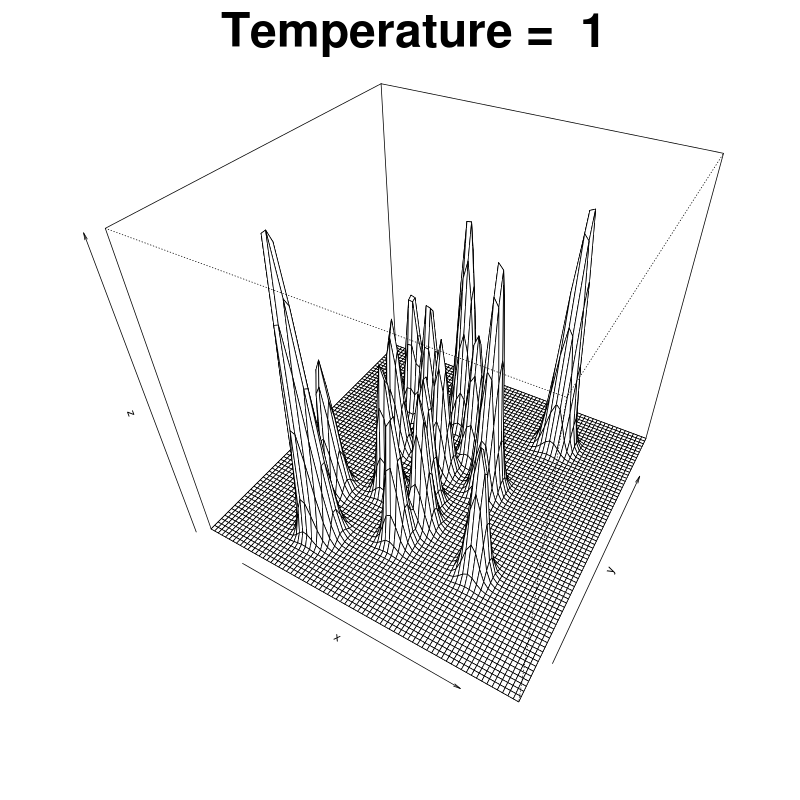
\includegraphics[scale=.3]{./picts/Liang_perspective.png}\end{figure}	
	\end{center}	
		
\end{frame}

\begin{frame}
		\frametitle{toy-example visualised as a contour plot}
	
	\begin{center}
		\begin{figure}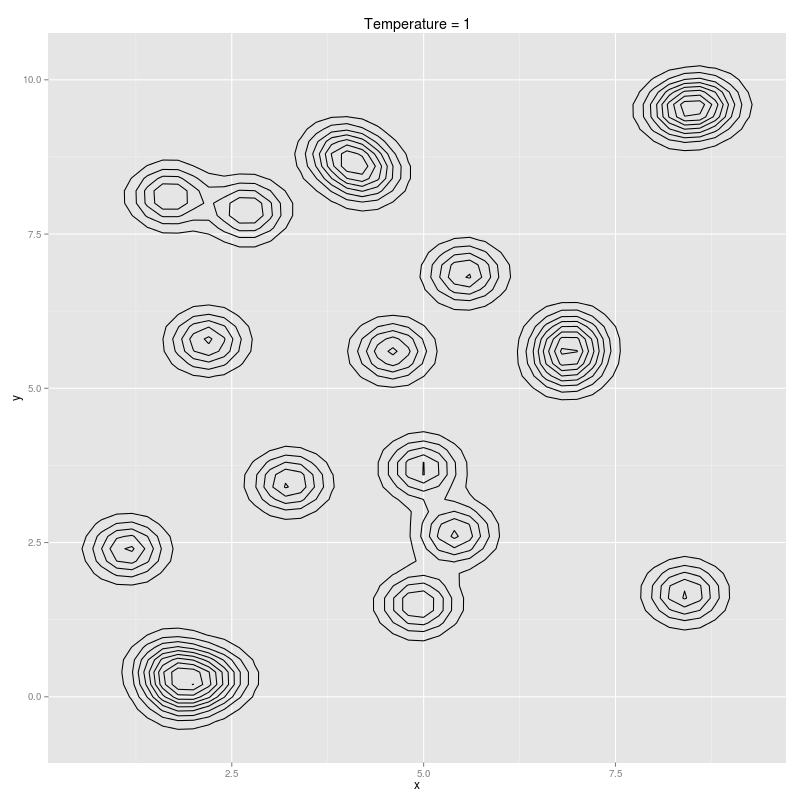
\includegraphics[scale=.25]{./picts/Liang_Contour_plot.png}\end{figure}	
	\end{center}	
		
\end{frame}

	%%%%%%%%%%%%%%%%%%%%%%%%%%%%%%%%%%%%%%%%%%%%%%%%%%%%%%%%%%%%%%

\begin{frame}[plain]

	\begin{center}
		\begin{figure}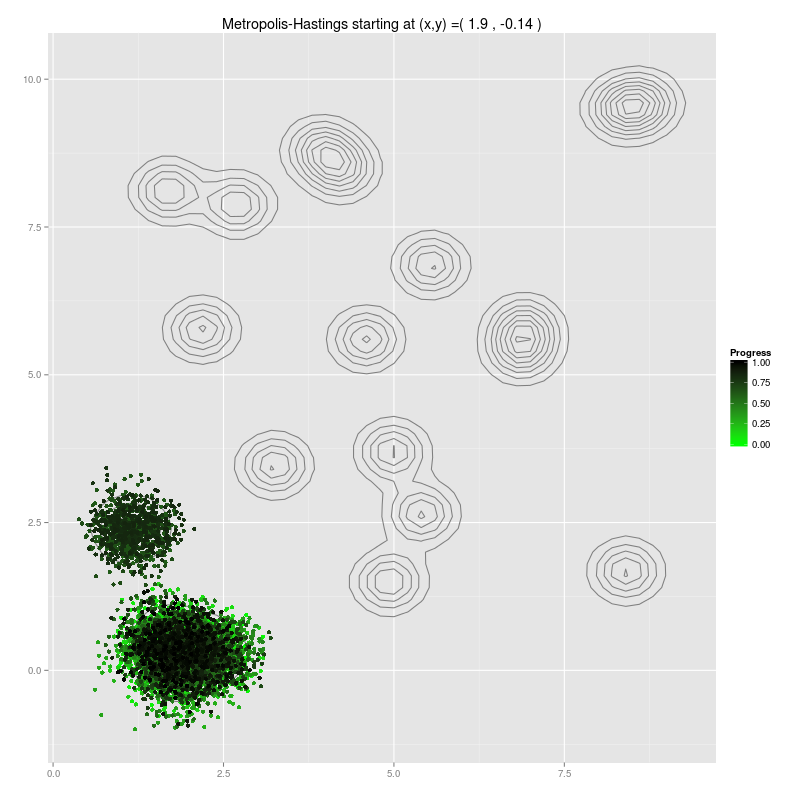
\includegraphics[scale=.31]{./picts/MH_simululation_10000_steps.png}\end{figure}	
	\end{center}	
		
\end{frame}

\begin{frame}[plain]

	\begin{center}
		\begin{figure}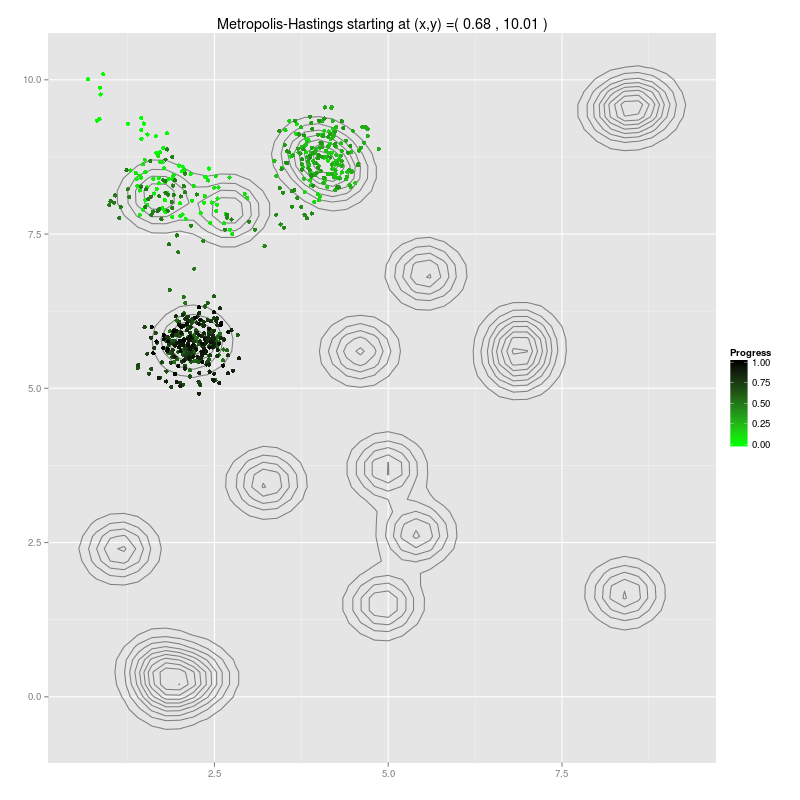
\includegraphics[scale=.31]{./picts/MH_simululation_1000_steps_ex1.png}\end{figure}	
	\end{center}	
		
\end{frame}

\begin{frame}[plain]

	\begin{center}
		\begin{figure}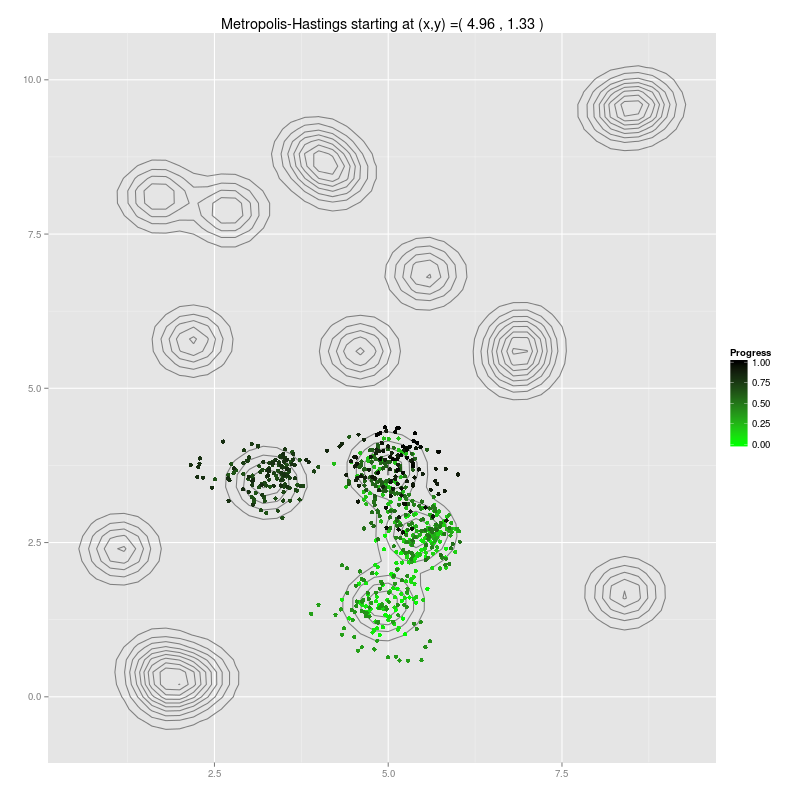
\includegraphics[scale=.31]{./picts/MH_simululation_1000_steps_ex2.png}\end{figure}	
	\end{center}	
		
\end{frame}

	%%%%%%%%%%%%%%%%%%%%%%%%%%%%%%%%%%%%%%%%%%%%%%%%%%%%%%%%%%%%%%


\begin{frame}
	\frametitle{Parallel Tempering in action.}
	\begin{center}
		\begin{figure}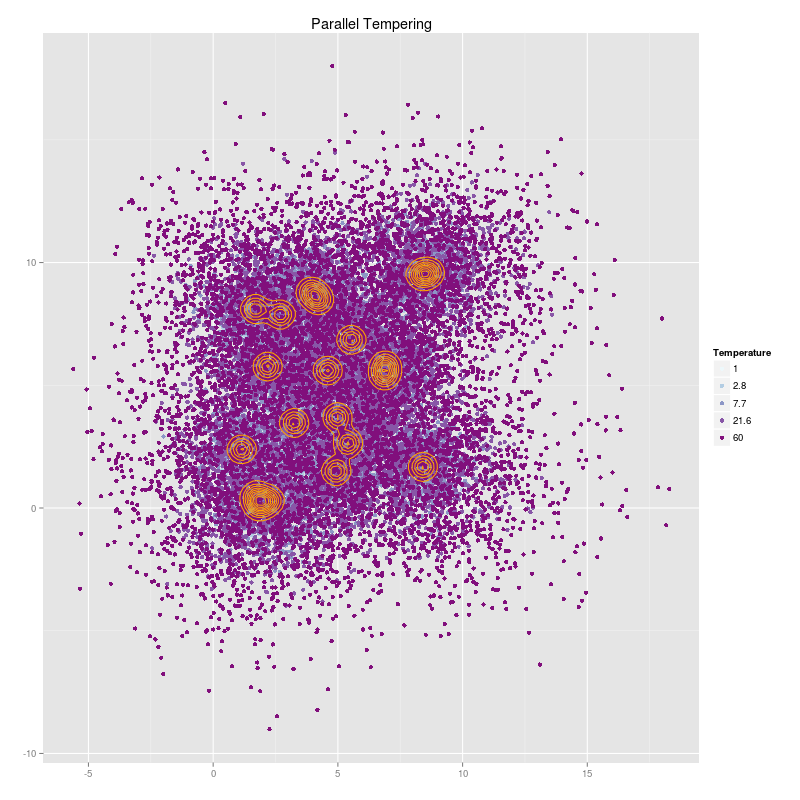
\includegraphics[scale=.28]{./picts/PT_simululation_10000_steps_1.png}\end{figure}	
	\end{center}	
		
\end{frame}


	
	\section[Theory]{Theory of Parallel Tempering}
		%%%%%%%%%%%%%%%%%%%%%%%%%%%%%%%%%%%%%%%%%%%%%%%%%%%%%%%%%%%%%%%%%%%%%%%%%%%%%%%%%%%%%%%%%%%%%%%%%%%%%%%%%%%
		\subsection{Notation}
%%%%%%%%%%%%%%%%%%%%%%%%%%%%%%%%%%%%%%%%%%%%%%%%%%%%%%%%%%%%%%%%%%%%%%%%%%%%%%%%%%%%%%%%%%%%%%%%%%%%%%%%%%%


\begin{frame}
		\frametitle{Getting inside Parallel Tempering}
	
	\begin{center}
	\begin{tabular}{cc}
		$(\Omega, \mathfrak{F})$ & measurable space \\ 
		 
		$\Omega$ & subset of a Polish space \\ 
		 
		$\mathfrak{F}$ & Borel subsets countably generated\\ 
		 
		$\mathcal{I} = [0,1]$ & unit interval \\ 
		 
		$ \pi: \mathfrak{F} \mapsto \mathcal{I}$ & measure \\ 
	\end{tabular} 	


		\begin{figure}\includegraphics[scale=.3, keepaspectratio]{./picts/nutshell2.jpg}\end{figure}	
	\end{center}

\end{frame}


%%%%%%%%%%%%%%%%%%%%%%%%%%%%%%%%%%%%%%%%%%%%%%%%%%%%%%%%%%%%%%%%%%%%%

\begin{frame}
		\frametitle{Assumptions and further notation}
	
	\begin{itemize}
		\item[\textcolor{green}{As.}] $\pi$ has density w.r. to Lebesgue measure
		\item $\pi$ - the density
		\begin{itemize}
			\item know up to its proportionality factor
			\item unnormalised
		\end{itemize}
	\end{itemize}	

	 $$ \int_{\Omega} \pi(x) \mathrm{d}\, x \in (0, \infty) $$
\end{frame}


%%%%%%%%%%%%%%%%%%%%%%%%%%%%%%%%%%%%%%%%%%%%%%%%%%%%%%%%%%%%%%%%%%%%%%%%%%%%%%%%%%%%%%%%%%%%%%%%%%%%%%%%%%%
		\subsection{Ideology}
%%%%%%%%%%%%%%%%%%%%%%%%%%%%%%%%%%%%%%%%%%%%%%%%%%%%%%%%%%%%%%%%%%%%%%%%%%%%%%%%%%%%%%%%%%%%%%%%%%%%%%%%%%%

\begin{frame}
		\frametitle{Solution's ideology}
	
	\begin{itemize}
			
		\item[] Space for chains
			 $$(\Omega^L, \mathfrak{F}^{\otimes L}, \pi_\beta)$$
		\item[]
		\item[] where $\mathfrak{F}^{\otimes L} \equiv \underbrace{\mathfrak{F} \otimes \dots \otimes \mathfrak{F}}_{\text{$L$ times}}$
		\item[]
		\item[] $$ \pi_\beta \propto \pi^{\beta_1} \times \dots \times \pi^{\beta_L} $$
		\item[]
		\item[] $\beta = (\beta_1 , \dots , \beta_L)$ - inverse temperatures $\beta_i = T_i^{-1}$
		\item[] and $1 = T_1 < \dots < T_L < \infty$	
		\item[]
		\item[]\emph{no normalisation of $\pi_\beta$ coordinates }	
	\end{itemize}	


\end{frame}

%%%%%%%%%%%%%%%%%%%%%%%%%%%%%%%%%%%%%%%%%%%%%%%%%%%%%%%%%%%%%%%%%%%%%

\begin{frame}
		\frametitle{\dots enters Markov}
	
	\begin{itemize}
			
		\item[] Markov Chain $X \equiv \{ X^{[k]}\}_{k \geq 0}$
		\begin{itemize}
			\item $\Omega^L$ state-space for $ X $
		\end{itemize}
		
		\item[]   $$X^{[k]} = (X_1^{[k]}, \dots, X_L^{[k]})$$
	\end{itemize}	

	\begin{center}
\begin{figure}\includegraphics[scale=1, keepaspectratio]{./picts/influence.pdf}\end{figure}	
	\end{center}
\end{frame}


%%%%%%%%%%%%%%%%%%%%%%%%%%%%%%%%%%%%%%%%%%%%%%%%%%%%%%%%%%%%%%%%%%%%%

\begin{frame}
		\frametitle{ non-Swedish way to equidistribution }
	
	\begin{itemize}
			
		\item[\textcolor{green}{As.}] $ \pi > 0$ somewhere between modes 
		
		\begin{itemize}
			\item then $\pi^{\beta_k} > \pi$ for $k \geq 2$
		\end{itemize}
		
		\item[] So that if $\pi(y) < \pi(x)$ then  
 $$\alpha_{\beta_1}(x,y) = 1 \wedge \frac{\pi(y)}{\pi(x)} = \frac{\pi(y)}{\pi(x)} <  \Big(\frac{\pi(y)}{\pi(x)}\Big)^{\beta_k} = 1 \wedge (\frac{\pi(y)}{\pi(x)})^{\beta_k} = \alpha_{\beta_k}(x,y)$$

		\begin{itemize}
			\item proposal accepted more often in higher temperatures when  $$\frac{\pi(y)}{\pi(x)} < 1$$
			\item we enlarge regions from which proposals get accepted
		\end{itemize}

	\end{itemize}	

\end{frame}


%%%%%%%%%%%%%%%%%%%%%%%%%%%%%%%%%%%%%%%%%%%%%%%%%%%%%%%%%%%%%%%%%%%%%%%%%%%%%%%%%%%%%%%%%%%%%%%%%%%%%%%%

\begin{frame}[plain]

	\begin{center}
		\begin{figure}\includegraphics[scale=.15]{./picts/Liang_perspectives.png}\end{figure}	
	\end{center}	
		
\end{frame}


\begin{frame}[plain]

	\begin{center}
		\begin{figure}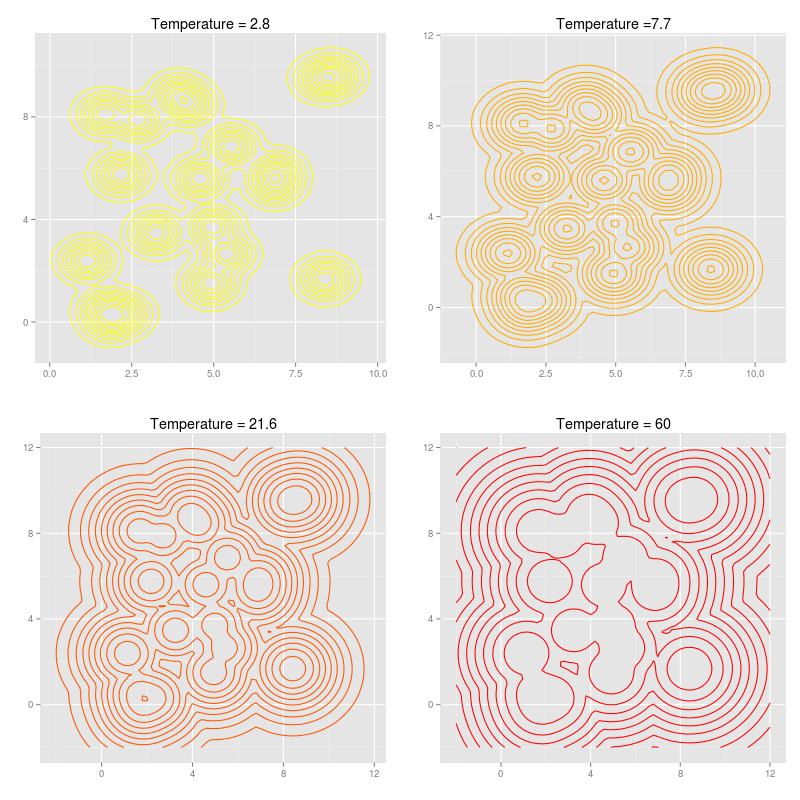
\includegraphics[scale=.31]{./picts/Liang_Contour_plots.png}\end{figure}	
	\end{center}	
		
\end{frame}

%%%%%%%%%%%%%%%%%%%%%%%%%%%%%%%%%%%%%%%%%%%%%%%%%%%%%%%%%%%%%%%%%%%%%

\begin{frame}
		\frametitle{ Potential Problems }

	\begin{center}
		\begin{figure}\includegraphics[scale=1, keepaspectratio]{./picts/probability_cloud1.pdf}\end{figure}	
	\end{center}
\end{frame}


%%%%%%%%%%%%%%%%%%%%%%%%%%%%%%%%%%%%%%%%%%%%%%%%%%%%%%%%%%%%%%%%%%%%%

\begin{frame}
		\frametitle{ Potential Problems }

	\begin{itemize}
		\item $\pi$ might be ok 
		\item because of computer's finite arithmetic it is not ok anymore
	\end{itemize}

\end{frame}


%%%%%%%%%%%%%%%%%%%%%%%%%%%%%%%%%%%%%%%%%%%%%%%%%%%%%%%%%%%%%%%%%%%%%

\begin{frame}
		\frametitle{ Theoretical Details }

	\begin{itemize}
		\item[] algorithm reached $n^\text{th}$ step - $X^{[n]}$
		\item[] we act with two kernels
 $$X^{[n]} \overset{\swap}{\rightarrow} \widetilde{X}^{[n +1]} \overset{\metro}{\rightarrow} X^{[n + 1]}.$$
		
		\item[]
		\item $\swap$ - swap kernel
		\item $\metro$ - random walk kernel
		\item[]
		\item Their reversibility is assured by the MHG algorithm reversibility. 
		\begin{itemize}
			\item[] so we get $\pi$-preservation 
			$$ \swap \metro \pi =  \swap \pi = \pi$$
		\end{itemize}
	\end{itemize}

\end{frame}
%%%%%%%%%%%%%%%%%%%%%%%%%%%%%%%%%%%%%%%%%%%%%%%%%%%%%%%%%%%%%%%%%%%%%%%%%%%%%%%%%%%%%%%%%%%%%%%%%%%%%%%%%%%
		\subsection{random walk kernel}
%%%%%%%%%%%%%%%%%%%%%%%%%%%%%%%%%%%%%%%%%%%%%%%%%%%%%%%%%%%%%%%%%%%%%%%%%%%%%%%%%%%%%%%%%%%%%%%%%%%%%%%%%%%

\begin{frame}
		\frametitle{ random walk $\metro$ }

	\begin{itemize}
		\item[] take $A_i \in \mathfrak{F}$ and $x \in \Omega^L$
		\item[] then
  $$\metro (x, A_1 \times \dots \times A_L) = \prod_{l=1}^L \metrobis{l}(x_l, A_l)$$
		
		\item[] where $\metrobis{l}(x_l, A_l)$ is equal to  
		\item[] 
$$\int_A \alpha_{\beta_l} (x_l, y_l) q_{\Sigma_l} (y_l - x_l) \mathrm{d }y_l + \delta_x (A) \int [1 - \alpha_{\beta_l} (x_l, y_l)] q_{\Sigma_l} (y_l - x_l) \mathrm{d }y_l$$

		\item[] where $\alpha_{\beta_l}$ is the acceptance level 
		\item[] and $q_{\Sigma_l}$ is proposal distribution 
	\end{itemize}

\end{frame}

%%%%%%%%%%%%%%%%%%%%%%%%%%%%%%%%%%%%%%%%%%%%%%%%%%%%%%%%%%%%%%%%%%%%%
\begin{frame}
		\frametitle{ Observations and assumptions }

	\begin{itemize}
		\item[\textcolor{green}{As.}] $q_{\Sigma_l}$ - density of $\mathcal{N}(0, \Sigma_l)$
		\item[]
		\item[] Symmetry $q(x_l,y_l) = q(y_l,x_l)$ implies 
		\item[]	$$ \alpha_{\beta_l} (x_l, y_l)  \equiv 1 \wedge \frac{\pi^{\beta_l}(y_l)}{\pi^{\beta_l}(x_l)} $$
		\item[] for the chain to preserve $\pi_\beta$.
		\item[] 
		\item[] Implementation: independent simulation of $\metrobis{l}$ for each $\widetilde{X}^{[n-1]}_l$
		
	\end{itemize}

\end{frame}

%%%%%%%%%%%%%%%%%%%%%%%%%%%%%%%%%%%%%%%%%%%%%%%%%%%%%%%%%%%%%%%%%%%%%%%%%%%%%%%%%%%%%%%%%%%%%%%%%%%%%%%%%%%
		\subsection{swap kernel}
%%%%%%%%%%%%%%%%%%%%%%%%%%%%%%%%%%%%%%%%%%%%%%%%%%%%%%%%%%%%%%%%%%%%%%%%%%%%%%%%%%%%%%%%%%%%%%%%%%%%%%%%%%%

\begin{frame}
		\frametitle{ Interlacing independent chains with $\swap$}

	\begin{itemize}
		\item[] Swaps
		\begin{itemize}
			\item Less-tempered chains placed in unusual places
			\item a pair of coordinates $(\widetilde{X}^{[n-1]}_l, \widetilde{X}^{[n-1]}_k)$ drawn at random
			\item[\textcolor{green}{As.}] only one pair per turn
			\item different strategies possible 
		\end{itemize}

		\item[] 
		\item[]	Introduce swap operation 
		$$S_{ij} x = (x_1, \dots, x_{i-1}, x_j, x_{i+1}, \dots, x_{j-1}, x_i, x_{j+1}, \dots, x_L)$$
	\end{itemize}

\end{frame}

%%%%%%%%%%%%%%%%%%%%%%%%%%%%%%%%%%%%%%%%%%%%%%%%%%%%%%%%%%%%%%%%%%%%%
\begin{frame}
		\frametitle{ Precise kernel form of $\swap$}

	\begin{itemize}
		\item[] For any $x \in \Omega^L$ and $A \in \mathfrak{F}^{\otimes L}$ 
	$$\swap(x, A) \equiv$$
		\item[]
$$\underset{ i < j}{\sum} p_{ij}(x) \alpha_\text{swap} (x, S_{ij}x) \mathbb{I}_A(S_{ij} x) + \Big( 1 - \underset{ i < j}{\sum} p_{ij}(x) \alpha_\text{swap} (x, S_{ij}x)\Big) \mathcal{I}(x,A)$$

		\item[] where 
$$\alpha_\text{swap}(x,S_{ij} x) = \Big[  \Big(\frac{\pi(x_j)}{\pi(x_i)} \Big)^{\beta_i - \beta_j}  \frac{ p_{ij}(S_{ij} x )}{ p_{ij}( x ) }\Big] \wedge 1$$
		\item[] is the acceptance level for swaps, 
		\item[] $p_{ij}( x )$ - probability function of a swap given $x$. 
		\item[] \emph{Nota bene:} given state $x$, $\swap$ has a finite support 
	$$\mathfrak{S}_x \equiv\{ S_{ij} x : i <j \}$$
	\end{itemize}

\end{frame}


		% Comparison to MHG algorithm.

	\section[Swaps]{Swapping Strategies}
		
\begin{frame}
		\frametitle{ Different possible swapping strategies $p_{ij}( x )$ }

	\begin{itemize}
		\item[] Strategy I 
		\item[] 
	$$p_{ij}(x) \propto \frac{\pi (x_j)}{\pi( x_i )} \wedge \frac{\pi (x_i)}{\pi( x_j )} = \exp \Big( - | \log ( \pi(x_j) ) - \log ( \pi(x_i) ) | \Big)$$
		\begin{itemize}		
 			\item promotes swaps between coordinates relatively the same,  $\pi (x_j) \approx \pi (x_i)$ 
		\end{itemize}
	
		\item[] Strategy II 
		\item[] 
	$$p_{ij}(x) \propto \frac{\pi (x_j)}{\pi (x_i)} \wedge 1 = \exp \Big( - ( \log ( \pi(x_j) ) - \log ( \pi(x_j) ) )\Big) \wedge 1$$
		\begin{itemize}		
 			\item breaks the symmetry of the previous one
		\end{itemize}

	\end{itemize}

\end{frame}

	% Strategy One
\begin{frame}[plain]

	\begin{center}
		\begin{figure}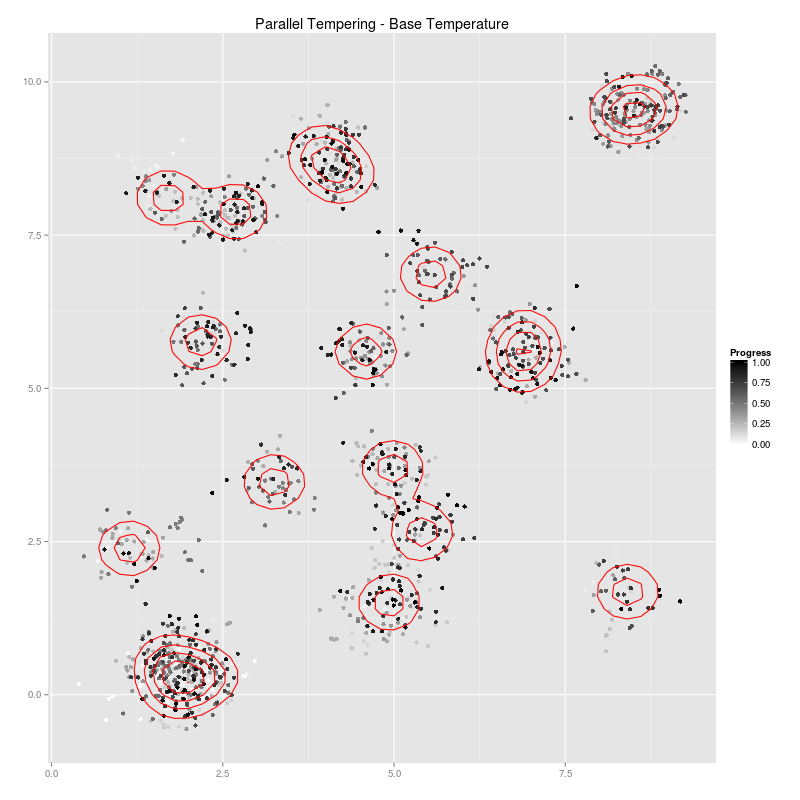
\includegraphics[scale=.31]{./picts/PT_simululation_base_temperature_2000_steps_strategy_1_try_1.png}\end{figure}	
	\end{center}	
		
\end{frame}


	% Strategy Two
\begin{frame}[plain]

	\begin{center}
		\begin{figure}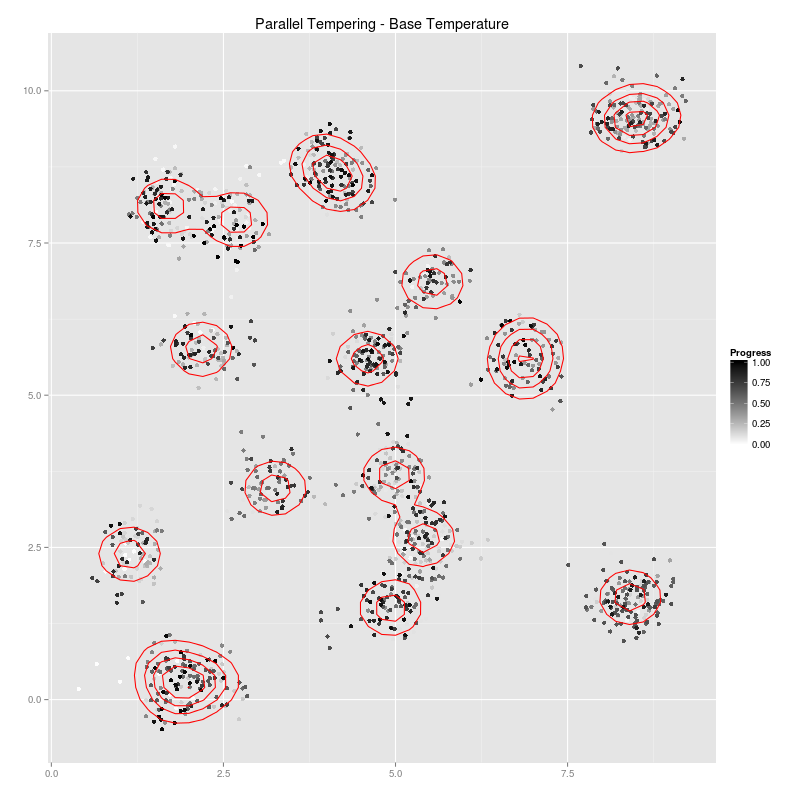
\includegraphics[scale=.31]{./picts/PT_simululation_base_temperature_2000_steps_strategy_2_try_1.png}\end{figure}	
	\end{center}	
		
\end{frame}


%%%%%%%%%%%%%%%%%%%%%%%%%%%%%%%%%%%%%%%%%%%%%%%%%%%%%%%%%%%%%%%%%%%%%
\begin{frame}
		\frametitle{ Different possible swapping strategies $p_{ij}( x )$ }

	\begin{itemize}
		\item[] Strategy III 
		\item[] 
	$$p_{ij} \propto \Big( \frac{\pi (x_j)}{\pi( x_i )} \wedge \frac{\pi (x_i)}{\pi( x_j )} \Big)^{\beta_i - \beta_j} = \exp \Big( - (\beta_i - \beta_j)| \log ( \pi(x_j) ) - \log ( \pi(x_i) ) | \Big)$$
		\begin{itemize}		
 			\item softens the requirement  $\pi (x_j) \approx \pi (x_i)$
			\item promotes $\beta_i - \beta_j \approx 0$ 
			\item promotes swaps between adjacent chains 
		\end{itemize}
	
		\item[] Strategy IV 
		\item[] 
	$$p_{ij} \propto \Big( \frac{\pi (x_j)}{\pi( x_i )} \wedge \frac{\pi (x_i)}{\pi( x_j )} \Big)^\frac{\beta_i - \beta_j}{1 + \rho(x_i, x_j)} = \exp \Big( - \frac{(\beta_i - \beta_j)| \log ( \pi(x_j) ) - \log ( \pi(x_i) ) |}{{1 + \rho(x_i, x_j)}} \Big)$$
		\begin{itemize}		
 			\item added a quasi-metric 
			\item $\rho$ does not require symmetry $\rho(x_i, x_j) = \rho(x_j, x_i)$  
			\item could be of use in the Gibbs random-field model
		\end{itemize}

	\end{itemize}

\end{frame}

	% Strategy Three

\begin{frame}[plain]

	\begin{center}
		\begin{figure}\includegraphics[scale=.31]{./picts/PT_simululation_base_temperature_2000_steps_strategy_3_try_1.png}\end{figure}	
	\end{center}	
		
\end{frame}

	% Strategy Four

\begin{frame}[plain]

	\begin{center}
		\begin{figure}\includegraphics[scale=.31]{./picts/PT_simululation_base_temperature_1000_steps_1.png}\end{figure}	
	\end{center}	
		
\end{frame}

\begin{frame}[plain]

	\begin{center}
		\begin{figure}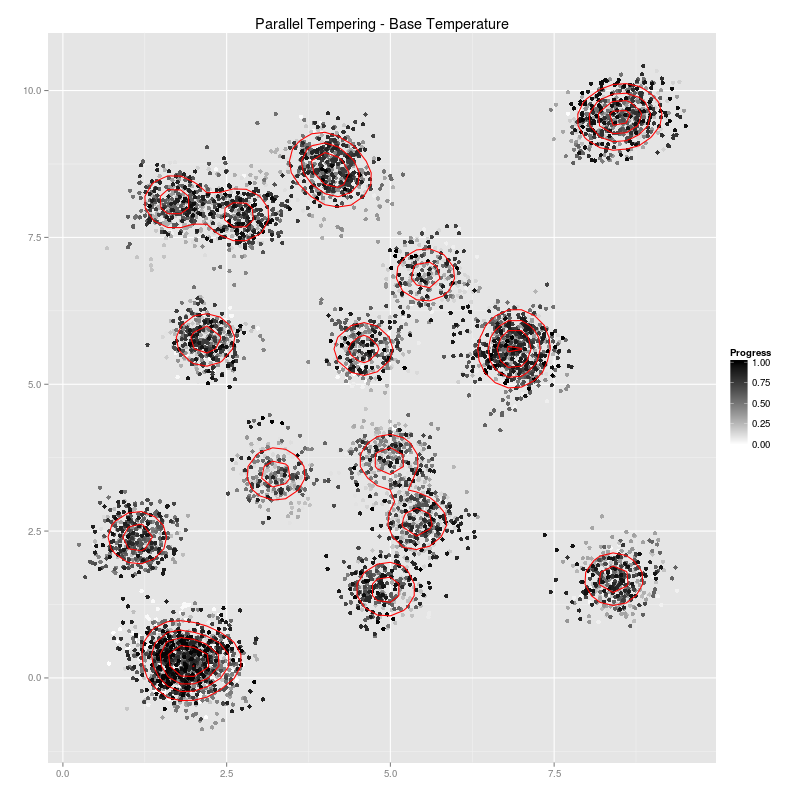
\includegraphics[scale=.31]{./picts/PT_simululation_base_temperature_10000_steps_1.png}\end{figure}	
	\end{center}	
		
\end{frame}




 	% Swapping strategies. 

	\section[Sources]{Bibliography}
		\begin{frame}

	\frametitle{Bibliography}
	
	
	\begin{thebibliography}{10}

		\beamertemplatearticlebibitems

			\bibitem{promo}
	  			Błażej Miasojedow, Eric Moulines, Matti Vihola,
	 			\emph{Adaptive Parallel Tempering Algorithm},
	  			Arxive.

			\bibitem{equi_energy_moves}  
				Meïli Baragatti, Agnès Grimaud, Denys Pommeret
				\emph{Parallel Tempering with Equi-Energy Moves}.  

		
		\beamertemplatebookbibitems
		
			\bibitem{geyer}  
				Charles J. Geyer,
				\emph{Markov Chain Monte Carlo Lecture Notes}. 
	

	\end{thebibliography}

\end{frame}



	%%%%%%%%%%%%%%%%%%%%%%%%%%%%%%%%%%%%%%%%%%%%%%%%%%%%%%%%%%%%%%

\end{document}
  
  
%%%%%%%%%%%%%%%%%%%%%%%%%%%%%%%%%%%%%%%%%%%%%%%%%%%%%%%%%%%%%%%%%%%%%%%%%%%

